\documentclass[tikz,border=4pt]{standalone}
\usepackage{amsmath,amssymb,bm}
\usetikzlibrary{positioning,arrows.meta,shapes.geometric,fit,calc}
\definecolor{cSo}{HTML}{1565C0}\definecolor{cAn}{HTML}{388E3C}\definecolor{cVei}{HTML}{F57C00}
\definecolor{cFn}{HTML}{7B1FA2}\definecolor{cPg}{HTML}{C62828}
\begin{document}
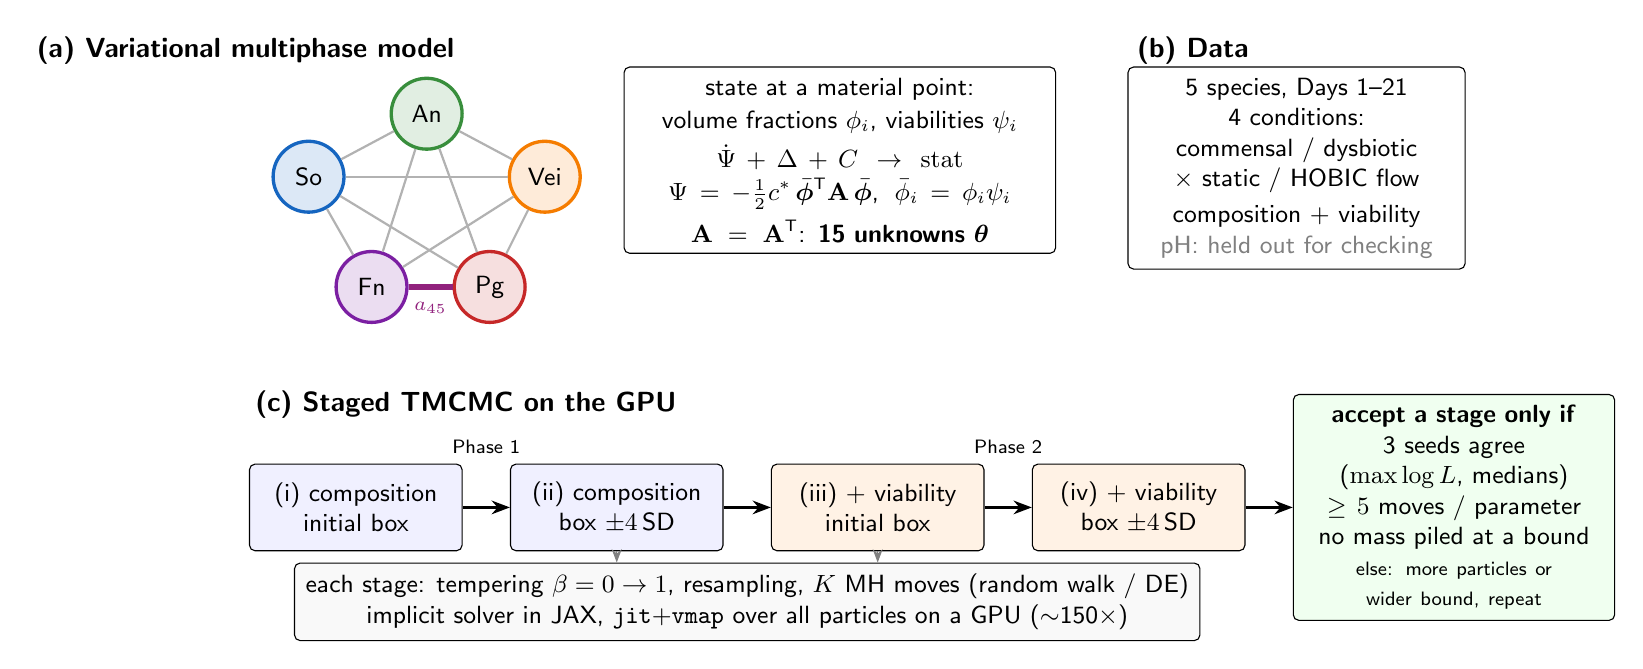
\begin{tikzpicture}[font=\sffamily\small,>=Stealth,
  sp/.style={circle,draw=#1,fill=#1!15,very thick,minimum size=9mm,inner sep=0pt},
  box/.style={draw,rounded corners=2pt,align=center,inner sep=4pt,fill=white},
  stage/.style={draw,rounded corners=2pt,align=center,minimum width=27mm,minimum height=11mm,inner sep=2pt},
  lab/.style={font=\sffamily\bfseries}]
% ---------- (a) model ----------
\node[lab] at (-0.2,3.2) {(a) Variational multiphase model};
\node[sp=cSo] (So) at (0.6,1.6) {So};
\node[sp=cAn] (An) at (2.1,2.4) {An};
\node[sp=cVei] (Vei) at (3.6,1.6) {Vei};
\node[sp=cFn] (Fn) at (1.4,0.2) {Fn};
\node[sp=cPg] (Pg) at (2.9,0.2) {Pg};
\foreach \a/\b in {So/An,So/Vei,An/Vei,So/Fn,An/Fn,Vei/Fn,So/Pg,An/Pg,Vei/Pg}{\draw[gray!60,thick] (\a)--(\b);}
\draw[cFn!70!cPg,line width=2.2pt] (Fn)--(Pg) node[midway,below=1pt,font=\sffamily\scriptsize] {$a_{45}$};
\node[box,anchor=north west,text width=52mm] at (4.6,3.0) {
  state at a material point:\\[1pt]
  volume fractions $\phi_i$, viabilities $\psi_i$\\[3pt]
  $\dot\Psi+\Delta+C\rightarrow\mathrm{stat}$\\[1pt]
  $\Psi=-\tfrac12 c^*\,\bar{\bm\phi}^{\mathsf T}\mathbf A\,\bar{\bm\phi}$,\; $\bar\phi_i=\phi_i\psi_i$\\[3pt]
  $\mathbf A=\mathbf A^{\mathsf T}$: \textbf{15 unknowns} $\bm\theta$};
% ---------- (b) data ----------
\node[lab,anchor=west] at (11.0,3.2) {(b) Data};
\node[box,anchor=north west,text width=40mm] (data) at (11.0,3.0) {
  5 species, Days 1--21\\
  4 conditions:\\ commensal / dysbiotic\\ $\times$ static / HOBIC flow\\[2pt]
  composition $+$ viability\\
  {\color{gray} pH: held out for checking}};
% ---------- (c) staged TMCMC ----------
\node[lab,anchor=west] at (-0.2,-1.3) {(c) Staged TMCMC on the GPU};
\node[stage,fill=blue!6] (s1) at (1.2,-2.6) {(i) composition\\ initial box};
\node[stage,fill=blue!6,right=6mm of s1] (s2) {(ii) composition\\ box $\pm4$\,SD};
\node[stage,fill=orange!10,right=6mm of s2] (s3) {(iii) $+$ viability\\ initial box};
\node[stage,fill=orange!10,right=6mm of s3] (s4) {(iv) $+$ viability\\ box $\pm4$\,SD};
\foreach \a/\b in {s1/s2,s2/s3,s3/s4}{\draw[->,thick] (\a)--(\b);}
\node[font=\sffamily\scriptsize,above=0mm of $(s1.north)!0.5!(s2.north)$] {Phase 1};
\node[font=\sffamily\scriptsize,above=0mm of $(s3.north)!0.5!(s4.north)$] {Phase 2};
\node[draw,rounded corners=2pt,fill=gray!5,inner sep=4pt,below=7mm of $(s2)!0.5!(s3)$,align=center] (gpu) {%
  each stage: tempering $\beta=0\to1$, resampling, $K$ MH moves (random walk / DE)\\
  implicit solver in JAX, \texttt{jit}$+$\texttt{vmap} over all particles on a GPU ($\sim$150$\times$)};
\draw[->,gray] (s2.south) -- (s2.south|-gpu.north);
\draw[->,gray] (s3.south) -- (s3.south|-gpu.north);
% ---------- (d) acceptance ----------
\node[box,right=6mm of s4,text width=38mm,anchor=west,fill=green!6] (acc) {
  \textbf{accept a stage only if}\\
  3 seeds agree ($\max\log L$, medians)\\
  $\ge5$ moves / parameter\\
  no mass piled at a bound\\
  {\scriptsize else: more particles or wider bound, repeat}};
\draw[->,thick] (s4)--(acc);
\end{tikzpicture}
\end{document}
